
\section{Dominio cerrado (Popescu/World)}
\subsection{Introducción}

\begin{frame}
  \frametitle{Introducción}\fontsize{8.0pt}{8.0}\selectfont
  \begin{block}{Modelo teórico: tratabilidad semántica (Popescu et al.)}
    \begin{itemize}
          \item QADB: Question answering como interfaz para una base de datos
          \item \textbf{Tratabilidad semántica de una pregunta $q$ en el contexto de una DB $d$}.
          \item Funcionalidad acotada y soporte solo para el inglés.
    \end{itemize}
  \end{block}

  \begin{block}{Pregunta}<2->
      \textbf{When was Albert Einstein born?}
  \end{block}
  \begin{columns}<3->
      \begin{column}{.5\textwidth}
      \end{column}
      \begin{column}{.1\textwidth}
      \begin{tikzpicture}[>=stealth, rotate border/.style={shape border uses incircle, shape border rotate=270}]
              \node[rotate border=-40, fill=black, minimum height=.4cm, single arrow, single arrow head extend=.2cm, single arrow head indent=.1cm, inner sep=1.5pt] (arrow) {};
          \end{tikzpicture}
      \end{column}
      \begin{column}{.3\textwidth}
          %Question Answering
      \end{column}
      \begin{column}{.5\textwidth}

      \end{column}
  \end{columns}

  \begin{exampleblock}{Consulta SQL}<3->
\textbf{{\color{purple}SELECT} birth\_date \newline
      {\color{purple}FROM} scientists\newline
      {\color{purple}WHERE} name $=$ {\color{green}`Albert Einstein'}
      }
  \end{exampleblock}
  \begin{columns}<4->
      \begin{column}{.5\textwidth}
      \end{column}
      \begin{column}{.1\textwidth}
      \begin{tikzpicture}[>=stealth, rotate border/.style={shape border uses incircle, shape border rotate=270}]
              \node[rotate border=-40, fill=black, minimum height=.4cm, single arrow, single arrow head extend=.2cm, single arrow head indent=.1cm, inner sep=1.5pt] (arrow) {};
          \end{tikzpicture}
      \end{column}
      \begin{column}{.3\textwidth}
          %Question Answering
      \end{column}
      \begin{column}{.5\textwidth}

      \end{column}
  \end{columns}

  \begin{alertblock}{Respuesta}<4->
      \textbf{March 14th, 1879}
  \end{alertblock}

\end{frame}



\subsubsection*{Base de datos}\fontsize{9.5pt}{8.2}\selectfont
\begin{frame}
\frametitle{Base de datos: World (Country, City y CountryLanguage)}
\begin{figure}
    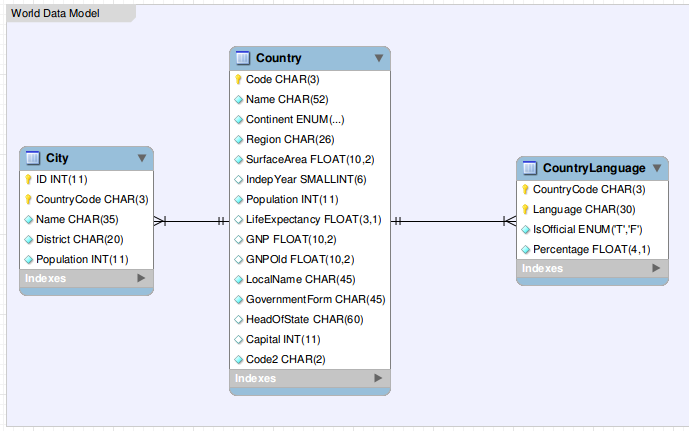
\includegraphics[width=9.823cm,height=6.004cm]{graficos/fuentes/world-db.png}
\end{figure}
\end{frame}



\subsection{Modelo teórico}


\begin{frame}[<+->]
  \frametitle{Tratabilidad semántica / motivación}
      \begin{itemize}
          \item La complejidad de las preguntas en lenguaje natural es arbitraria.
          \item Distinguir un subconjunto 1) \textit{tratable} y 2) \textit{abarcativo}
          \begin{itemize}
            \item La {\color{blue}\textbf{tratabilidad semántica}} formaliza ese conjunto simple y abarcativo
          \end{itemize}
          \item Rechazar y pedir reformulación de las no tratables
          \begin{itemize}
            \item Es mejor no dar respuesta a dar una mala. 
            \item Conservar la confianza en el sistema.
          \end{itemize}
      \end{itemize}
\end{frame}

\begin{frame}[<+->]
  \frametitle{Tratabilidad semántica / ejemplos}
    \begin{block}{Ejemplos}
      \begin{enumerate}
          \item ¿Qué países asiáticos son monarquías? $\rightarrow$ {\color{green}Sí}
          \item ¿Qué países de Asia no desarrollaron formas de gobierno basadas en las ideas de la Ilustración? $\rightarrow$ {\color{red}No}
          %\item ¿Qué países del continente de Lenin son monarquías? $\rightarrow$ {\color{red}No}
          \item ¿Qué países asiáticos tienen como gobierno una monarquía? $\rightarrow$ {\color{green}Sí}
          \item ¿Qué países del continente asiático tienen como forma de gobierno una monarquía? $\rightarrow$ {\color{green}Sí}
          \item ¿Qué países del continente que está al este de Europa y contiene a Rusia tiene esa forma de gobierno en la que manda una sola persona? $\rightarrow$ {\color{red}No}
      \end{enumerate}
    \end{block}
\end{frame}

\fontsize{7.0pt}{6.0}\selectfont
\begin{frame}[<+->]
  \frametitle{Tratabilidad semántica / intuición}
    \begin{block}{Una pregunta semánticamente tratable tiene:}
      \begin{itemize}
          \item {\color{blue}Atributos} y {\color{blue}Valores} apareados
          \item {\color{red}Valores} sueltos (atributo implícito)
          \item Una {\color{green}Q-word} (Qué, quién, cuándo) apareada con un atributo o suelta (atributo implícito)
          \item Marcadores sintácticos
          \item {\color{orange}Menciones sueltas a relaciones}
      \end{itemize}
    \end{block}
    \begin{exampleblock}{Abarcativo e intuitivamente traducible a una consulta SQL}
      \begin{itemize}
          \item ¿{\color{green}Qué} {\color{orange}países} del {\color{blue}continente} {\color{blue}asiático} tienen como {\color{blue}forma} de {\color{blue}gobierno} una {\color{blue}monarquía}?
            \begin{itemize}
              \item \fontsize{6pt}{5}\selectfont Debería ser algo como: {\color{purple}SELECT} Country.Name {\color{purple}FROM} Country {\color{purple}WHERE} Continent=\textbf{Asia} {\color{purple}AND} GovernmentForm=\textbf{Monarchy}
            \end{itemize}
            \item ¿{\color{green}Qué} {\color{orange}países} {\color{red}asiáticos} son {\color{red}monarquías}?
            \begin{itemize}
              \item \fontsize{6pt}{5}\selectfont Misma query, pero los atributos implícitos
            \end{itemize}
            \item ¿{\color{green}Quiénes} son los {\color{green}líderes} de las {\color{red}monarquías} {\color{red}asiáticas}?
            \begin{itemize}
              \item  \fontsize{6pt}{5}\selectfont Q-word apareada explicitamente con atributo: {\color{purple}SELECT} Country.HeadOfState {\color{purple}FROM} Country {\color{purple}WHERE} Continent=\textbf{Asia} {\color{purple}AND} GovernmentForm=\textbf{Monarchy}
            \end{itemize}
      \end{itemize}
    \end{exampleblock}
    
\end{frame}

\subsection{Implementación}


\begin{frame}[<+->]\fontsize{7.5pt}{7.2}\selectfont
  \frametitle{Módulos principales}
  \begin{block}{Lexicón: dominio semántico}
    \begin{itemize}
      \item Elementos de la DB $\rightarrow$ Wordnet $\rightarrow$ Lexicón (sinónimos)
      \item Todas las palabras que el sistema entiende están en el lexicón (tokens)
      \item Salto de las palabras a los elementos de la DB
      \begin{itemize}
        \item  \tiny{region, part, area, neighborhood, realm  $\rightarrow$ Atributo Country.Region  }
        \item  \tiny{city, metropolis, urban center  $\rightarrow$ Relación (tabla) City}
      \end{itemize}
    \end{itemize}
  \end{block}
  \begin{alertblock}{Tokenizer: pregunta $\rightarrow$ tokens del lexicón}
      \begin{itemize}
          \item Pregunta $q$ $\rightarrow$ Marcadores sintácticos (se tiran) + términos del lexicón
          \item Si no se puede, la pregunta ya no es tratable
          \item Propone particiones de $q$ en items del lexicón (tokenizaciones completas)
      \end{itemize}
  \end{alertblock}
  \begin{exampleblock}{Matcher: (tokens $\rightarrow$ elementos) + apareo + desambiguación}
      \begin{itemize}
          \item Filtra tokenizaciones válidas (\dq{traducciones}) con max flow (grafos)
          \item Descubre atributos implícitos
          \item Genera pares de atributos y valores y un atributo con la qword
          \item Desambigua sobreyecciones token $\rightarrow$ elemento al maximizar el flujo
    \end{itemize} 
  \end{exampleblock}
\end{frame}


% \begin{frame}[<+->]
%   \frametitle{Modulos principales}
%   \begin{block}{Lexicón: dominio semántico}
%     \begin{itemize}
%       \item Elementos de la DB $\rightarrow$ Wordnet $\rightarrow$ Lexicón (sinónimos)
%       \item \textbf{Elementos} de una DB: Relaciones, Atributos y Valores
%       \item Cada item del lexicón se llama \textbf{token}
%       \item Cada token es un sinónimo para uno o más elementos de la base de datos (\textbf{\dq{se corresponde con}})
%       \begin{itemize}
%             \item Esta relación va a ser el \dq{salto} entre las palabras y los elementos de la DB
%           \end{itemize}
%       \item Una pregunta \textit{tratable} va a constar de \textit{tokens} + marcadores sintácticos
%       %\item \fontsize{7.5pt}{7.2}\selectfont Notas: TokenAugmenter. Polisemia. Problemas.
%     \end{itemize}
%   \end{block}
%   \begin{alertblock}{Tokenizer}
%       \begin{itemize}
%           \item Elimina marcadores sintácticos
%           \item Rompe la pregunta y consulta al lexicón (¿a qué tokens pertenece esta palabra?)
%           \item Genera todas las particiones posibles de la pregunta en tokens del lexicón 
%           \begin{itemize}
%             \item Cada partición en tokens se llama \textit{tokenización completa}
%           \end{itemize}
%       \end{itemize}
%     \end{alertblock}
    
%     \begin{exampleblock}{Matcher}<1->
%       \begin{itemize}
%           \item Elimina marcadores sintácticos
%           \item Rompe la pregunta y consulta al lexicón (¿a qué tokens pertenece esta palabra?)
%           \item Genera todas las particiones posibles de la pregunta en tokens del lexicón 
%           \begin{itemize}
%             \item Cada partición en tokens se llama \textit{tokenización completa}
%           \end{itemize}
%       \end{itemize}
%     \end{exampleblock}
% \end{frame}


% \fontsize{9.5pt}{7.2}\selectfont
% \begin{frame}[<+->]
%   \frametitle{qword, compatibilidad}
%    \begin{itemize}
      
%       \item \textbf{Qwords} - pronombres interrogativos
%       \begin{itemize}
%         \item \{What, where, which, when, who\}, \{Qué, dónde, cuál, cuándo, quién\}
%         \item Funcionan como valores especiales (el valor preguntado)
%       \end{itemize}
%       \item \textbf{Compatibilidad}
%       \begin{itemize}
%           \item Valor $\rightarrow$ Atributo (Macri $\rightarrow$ HeadOfState)
%           \item Atributo  $\rightarrow$  Relación (HeadOfState $\rightarrow$ Country)
%           \item Valor $\rightarrow$ Relaciones de sus atributos (Macri $\rightarrow$ Country)
%           \item {\color{blue}Q-words $\rightarrow$ Atributos} (A manos)
%           \begin{itemize}
%             \item Who $\rightarrow$ HeadOfState, When $\rightarrow$ IndependenceYear , What $\rightarrow$ Varios atributos.
%           \end{itemize}
%       \end{itemize}
%     \end{itemize}
% \end{frame}


% \begin{frame}[<+->]
% \frametitle{Tokenización completa}

% \begin{block}{\textbf{Tokenización completa de una pregunta \textit{q}}}
%   \begin{itemize}
%     \item Una partición de tokens de la pregunta $q$
%     \item Pregunta tratable $\Leftrightarrow$ Marcadores sintácticos + tokens del lexicón
%    \end{itemize}
% \end{block}


% \end{frame}


% \fontsize{11pt}{7.2}\selectfont
% \begin{frame}
% \frametitle{Ejemplo}
% \begin{figure}
%   \centering
%     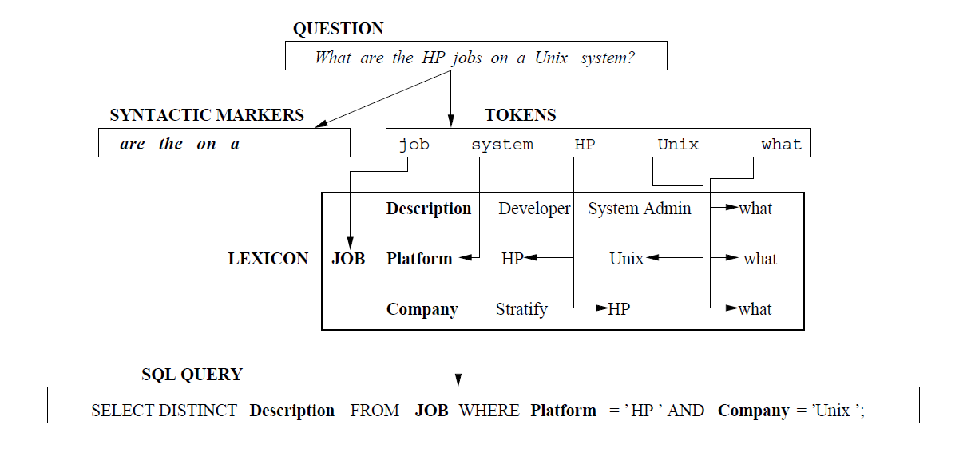
\includegraphics[scale=.7]{graficos/popescu-example}
%   \caption{La traducción de la pregunta ``What are the HP jobs on a Unix system?'' a una consulta SQL}
%   \label{fig:popescu-example}
% \end{figure}
% \end{frame}

% \begin{frame}[<+->]
% \frametitle{Matcher}
   
%    \begin{block}{Matcher}
%      \begin{itemize}
%       \item Input
%       \begin{itemize}
%         \item El tokenizer generó una más particiones de $q$ en items del lexicón (tokenizaciones)
%         \item Cada item mapea a uno o más elementos de la DB.
%       \end{itemize}
%       \item El matcher filtra mapeos válidos (\dq{traducciones válidas})
%         \begin{itemize}
%           \item  Relaciona cada \textbf{valor} con un único \textbf{atributo}, implícito o explícito usando un algoritmo de max flow.
%            \item Cada {\color{blue}atributo} del mapeo tiene un {\color{blue}valor} o {\color{green}qword} compatible y sintácticamente asociado.
%         \end{itemize}
%     \end{itemize} 
%   \end{block}
  
%   \begin{itemize}
%     \item Las aristas implicadas en el flujo máximo asocian 
%     \begin{enumerate}
%       \item los tokens de valor y de atributo y los correspondientes elementos (valores y atributos, respectivamente) de la DB y 
%       \item pares de valores y atributos entre sí.
%     \end{enumerate}
%     \end{itemize}
          
% \end{frame}

% \subsection{Implementación}

% \begin{frame}
%   \frametitle{Ejemplo}

%   \begin{figure}
%     \centering
%       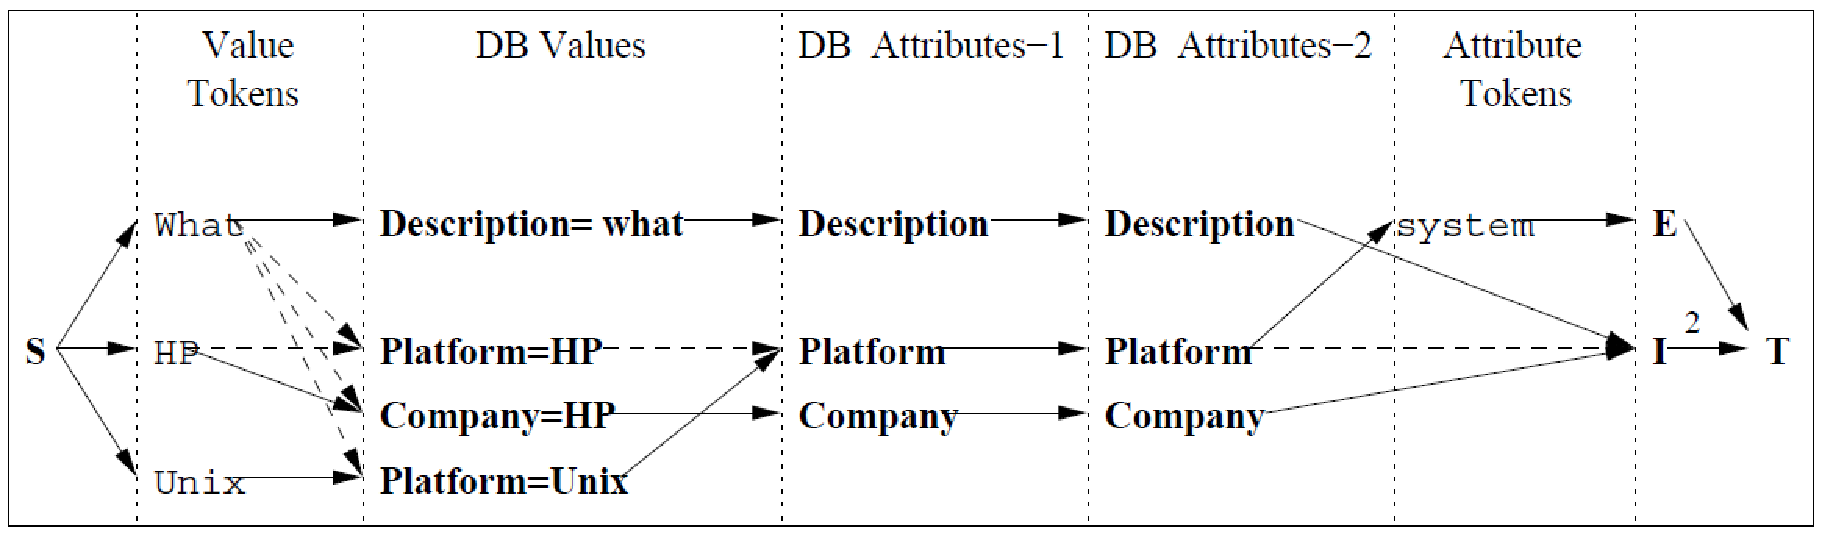
\includegraphics[scale=0.3]{graficos/popescu-example-2}
%     \caption{El grafo de atributos y valores del Matcher para la pregunta ``What are the HP jobs on a Unix system?''}
%     \label{fig:popescu-example-2}
%   \end{figure}

% \end{frame}

\begin{frame}[<+->] \fontsize{9.5pt}{8.2}\selectfont
    \frametitle{Traducción válida / Tratabilidad semántica}    
     Una \textbf{traducción válida} es un mapeo de una tokenización completa de $q$ en elementos de $E$ que cumple 3 condiciones:
    \begin{enumerate}
      \item Cada token se corresponde con un único elemento de $E$.
      \item Cada token de atributo se relaciona con un único token de valor, cumpliendo que:
      \begin{itemize}
        \fontsize{9.5pt}{7.2}\selectfont
        \item sus contrapartes del mundo DB son compatibles
        \item los dos tokens están sintácticamente asociados %\footnotemark 
       \end{itemize}
      \item Cada relación es compatible con algún atributo o valor
    \end{enumerate}

  \begin{alertblock}{Semánticamente tratable}
    Una pregunta es \textbf{semánticamente tratable} si tiene una q-word y al menos una traducción válida
  \end{alertblock}

    \begin{block}{Una traducción válida de $q$ se traduce trivialmente a una consulta SQL}        
    \begin{tabular}{ r | l }
    SELECT &  Atributo apareado con la qword \\
    WHERE & Pares de atributos y valores apareados (implícitos y explícitos)\\
    FROM & Todas las relaciones mencionadas \\
    \end{tabular}
    \end{block}


    %\footnotetext[1]{\tiny{Falta una condición sobre tokens de relación que no es esencial mencionar}}

\end{frame}

\fontsize{9.5pt}{8.2}\selectfont
\begin{frame}
\frametitle{Asociación sintáctica / Charniak parse tree}
\Tree [.S1 [.WHNP [.WP What ] ] [.SQ [.VP [.AUX are ] [.{\color{red}NP} [.DT the ] [.{\color{red}NNP} {\color{red}HP} ] [.{\color{red}NNS} {\color{red}jobs} ] ] [.PP [.IN on ] [.{\color{red}NP} [.DT a ] [.{\color{red}NNP} {\color{red}Unix} ] [.{\color{red}NN} {\color{red}system} ] ] ] ] ] [.. ? ] ] \\
{\color{red}Regla 1 - Sustantivos \dq{hermanos}}

\end{frame}

\begin{frame}
\frametitle{Asociación sintáctica / Charniak parse tree}
\Tree [.{\color{blue}S1} [.{\color{blue}WHNP} [.{\color{blue}WP} {\color{blue}What} ] ] [.{\color{blue}SQ} [.{\color{blue}VP} [.AUX are ] [.{\color{blue}NP} [.DT the ] [.{\color{blue}NNP} {\color{blue}HP} ] [.{\color{blue}NNS} {\color{blue}jobs} ] ] [.PP [.IN on ] [.NP [.DT a ] [.NNP Unix ] [.NN system ] ] ] ] ] [.. ? ] ] \\
{\color{blue}Regla 2: qwords a sustantivos}

\end{frame}


\subsubsection*{Ejemplos}

\begin{frame}[t]
\frametitle{Ejemplo 1: ``Who is the head of state of Zimbabwe?''}
Ejemplo 1:\newline
  \Large{``Who is the head of state of Zimbabwe?''}
\end{frame}

\begin{frame}[t]
\frametitle{Ejemplo 1: Tokenizer}
1. Separar, sacar puntuaciones, pasar a lower case, tirar stopwords:\newline
  \Large{\{{\color{blue}w}ho, {\color{red}\st{is}}, {\color{red}\st{the}}, head, {\color{red}\st{of}}, state, {\color{red}\st{of}}, {\color{blue}z}imbabwe\}}
\end{frame}


\begin{frame}[t]
\frametitle{Ejemplo 1: Tokenizer}
1. Separar, sacar puntuaciones, pasar a lower case, tirar stopwords:\newline
  \Large{\{who, head, state, zimbabwe\}}
\end{frame}

\begin{frame}[t]
\frametitle{Ejemplo 1: Tokenizer - tokens para who}
2. Obtener tokens para cada lema \tiny{(items del lexicón, sinónimo de 1+ elementos de la DB)} \newline
    \Large{$getTokens(who)\ \rightarrow \{$'who'$\}$}
\end{frame}

\begin{frame}[t]
\frametitle{Ejemplo 1: Tokenizer - tokens para head}
2. Obtener tokens para cada lema \newline
    \Large{$
    getTokens(head)\ \rightarrow \{$ 'head country', 'head teacher body politic', 'head body politic', 'head teacher land', 'read / write head dos', 'heading provincial', 'heading state', 'heading commonwealth', 'read / write head body politic', 'head word land', 'head state of matter', 'read / write head provincial', 'read / write head state department', 'head province',  'heading res publica', 'read / write head nation', (51 más)...$\}$}
\end{frame}

\begin{frame}[t]
\frametitle{Ejemplo 1: Tokenizer - tokens para state}
2. Obtener tokens para cada lema \newline
  \Large{ $getTokens(state)\ \rightarrow  \{$'heart eastern united states', 'centre eastern united states', 'central eastern united states', 'centrical eastern united states', 'midsection eastern united states', 'midriff eastern united states', 'centric eastern united states', 'center eastern united states', 'north western united states', (702 más)...$\}$}
\end{frame}

\begin{frame}[t]
\frametitle{Ejemplo 1: Tokenizer - tokens para Zimbabwe}
2. Obtener tokens para cada lema \newline
  \Large{$getTokens(zimbabwe)\ \rightarrow \{$'zimbabwe', 'republic of zimbabwe', 'capital of zimbabwe'$\}$}

\end{frame}

\begin{frame}[t]
\frametitle{Ejemplo 1: Tokenizer - intersección}
3. Filtrar solo tokens cuyos lemas estén en la pregunta\newline
  \Large{$getTokens(zimbabwe)\ \rightarrow \{$'zimbabwe', {\color{red}\st{'republic of zimbabwe'}}, {\color{red}\st{'capital of zimbabwe'}}$\}$ }
\end{frame}


\begin{frame}[t]
\frametitle{Ejemplo 1: Tokenizer - intersección}
3. Filtrar solo tokens cuyos lemas estén en la pregunta\newline
  \Large{
    $getTokens(zimbabwe) \rightarrow \{$'zimbabwe'$\}$\newline
    $getTokens(who)\ \rightarrow \{$'who'$\}$\newline
    $getTokens(head) \rightarrow \{$'head state'$\}$\newline
    $getTokens(state) \rightarrow  \{$'state','head state'$\}$
}
\end{frame}

\begin{frame}[t]
\frametitle{Ejemplo 1: ``Who is the head of state of Zimbabwe?''}
 5. Generar el conjunto de partes de todos contra todos (\textit{tokenizaciones}).\newline
  \Large{
      \{'state', 'zimbabwe'\},\newline
      \{ 'who', '{\color{red}state}', 'head {\color{red}state}', 'zimbabwe'\},\newline
      \{ 'who', 'head state', 'zimbabwe'\},\newline
      ...
  }\newline

\normalsize{
\begin{block}{Tokenización completa}  
  Quedarse solo con los que:
  \begin{itemize}
    \item Cubren la palabras no stopwords de la pregunta
    \item No tienen palabras {\color{red}repetidas}
  \end{itemize}
  
\end{block}
}
\end{frame}

\begin{frame}
\frametitle{Ejemplo 1: Tokenizaciones completas}

\begin{center}

$q = \text{``Who is the head of state of Zimbabwe?''}$
\end{center}
 \begin{equation*}
    CompleteTokenizations(q) = \begin{cases}
               \{\text{who, head state, zimbabwe}\}\} \\
           \end{cases}
\end{equation*}

\end{frame}

\begin{frame}[t]
\frametitle{Ejemplo 1: Lexicón - Tokens $\rightarrow$ Elementos}
Obtener elementos de la DB para cada token\newline
  \Large{
    $who \rightarrow Who$ (Qword compatible con HeadOfState) \newline
    $\text{head state} \rightarrow HeadOfState$ (Atributo de Country) \newline
    $zimbabwe \rightarrow Zimbabwe$ (Valor de Country.Name)\newline
    }
\end{frame}

\begin{frame}
\frametitle{Ejemplo 1: Matcher - Grafo de atributos y valores}
\begin{figure}
  \centering
    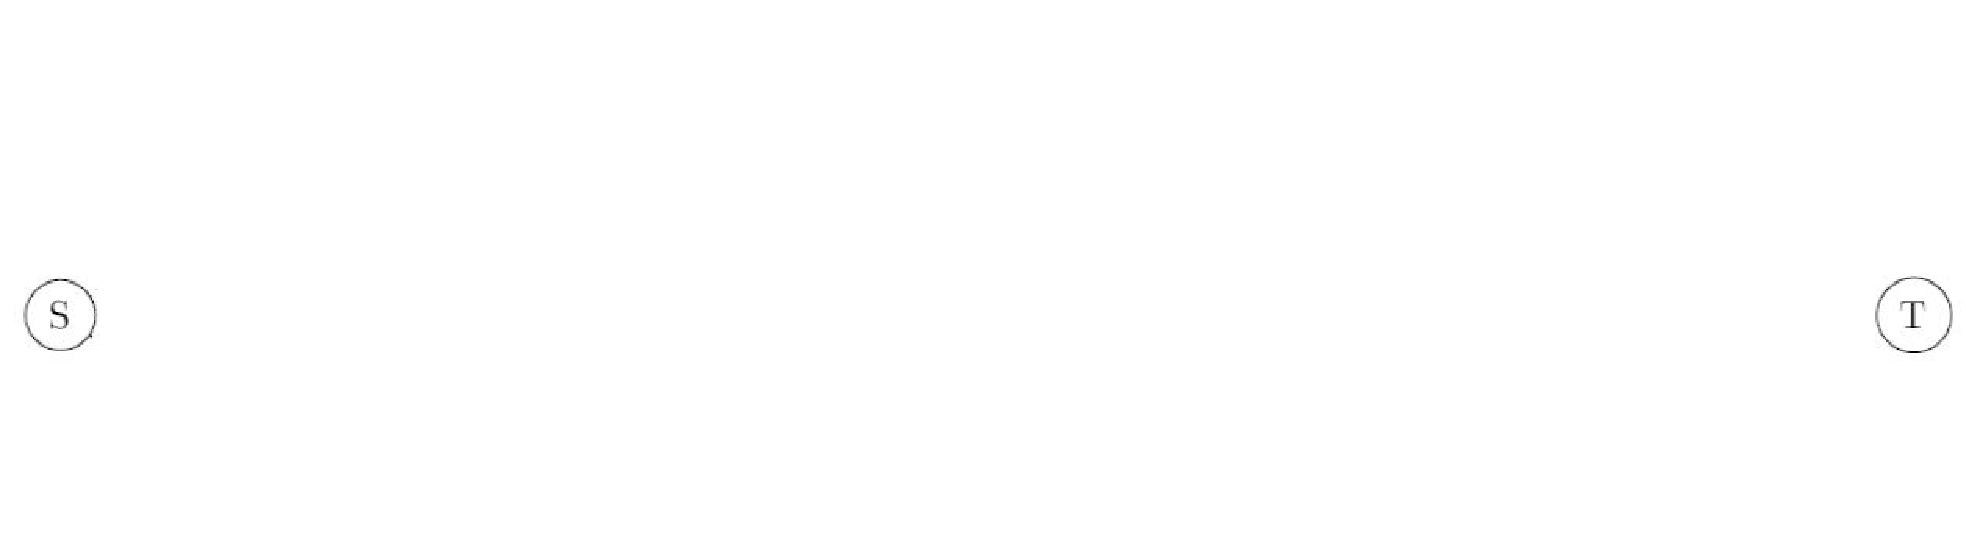
\includegraphics[scale=.33]{graficos/presentacion/ejemplo-grafo-matcher-1-2}
    \caption{1. Nodos Fuente (S) y Sumidero (T)}
\end{figure}

\end{frame}

\begin{frame}
\frametitle{Ejemplo 1: Matcher - Grafo de atributos y valores}
\begin{figure}
  \centering
    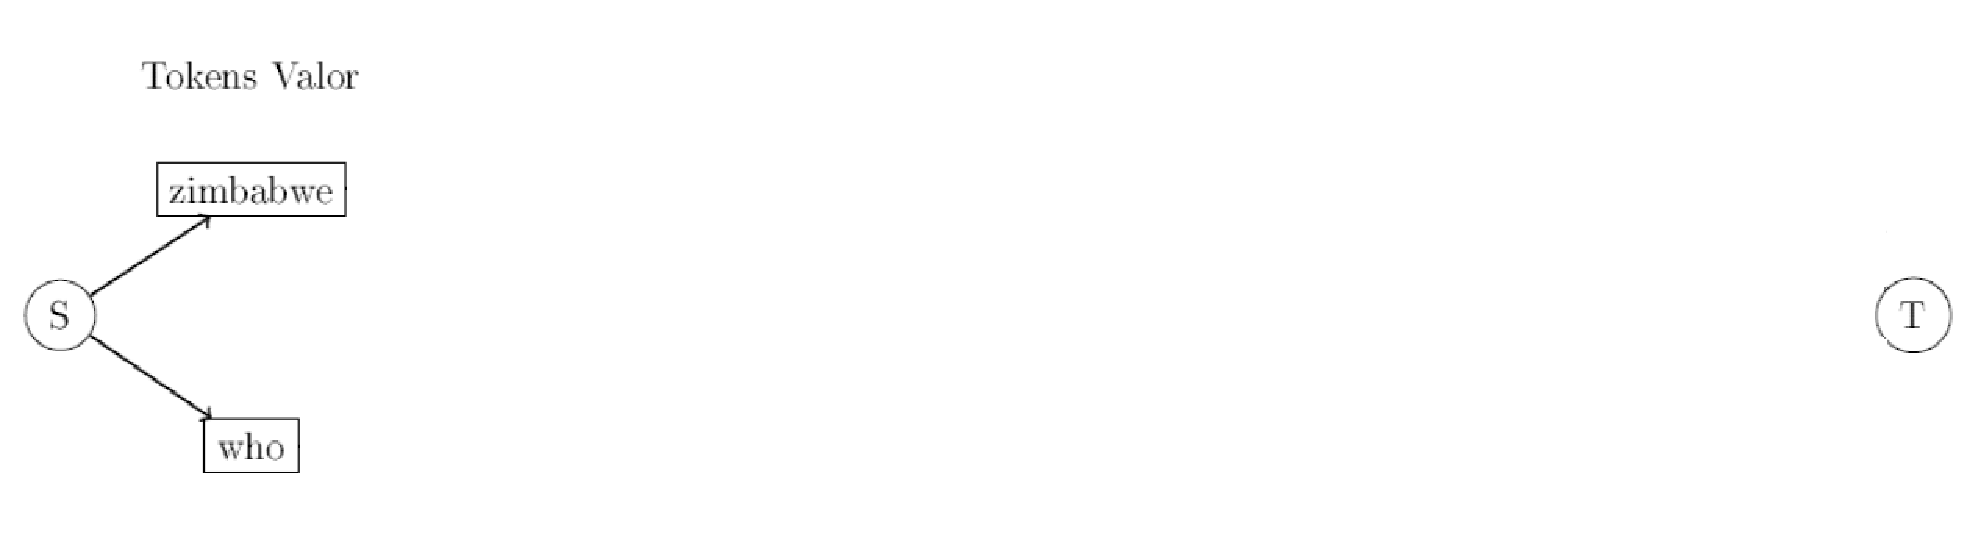
\includegraphics[scale=.33]{graficos/presentacion/ejemplo-grafo-matcher-1-3}
    \caption{2. Tokens de valor (palabras), desde S, con $f=1$}
\end{figure}
\end{frame}

\begin{frame}
\frametitle{Ejemplo 1: Matcher - Grafo de atributos y valores}
\begin{figure}
  \centering
    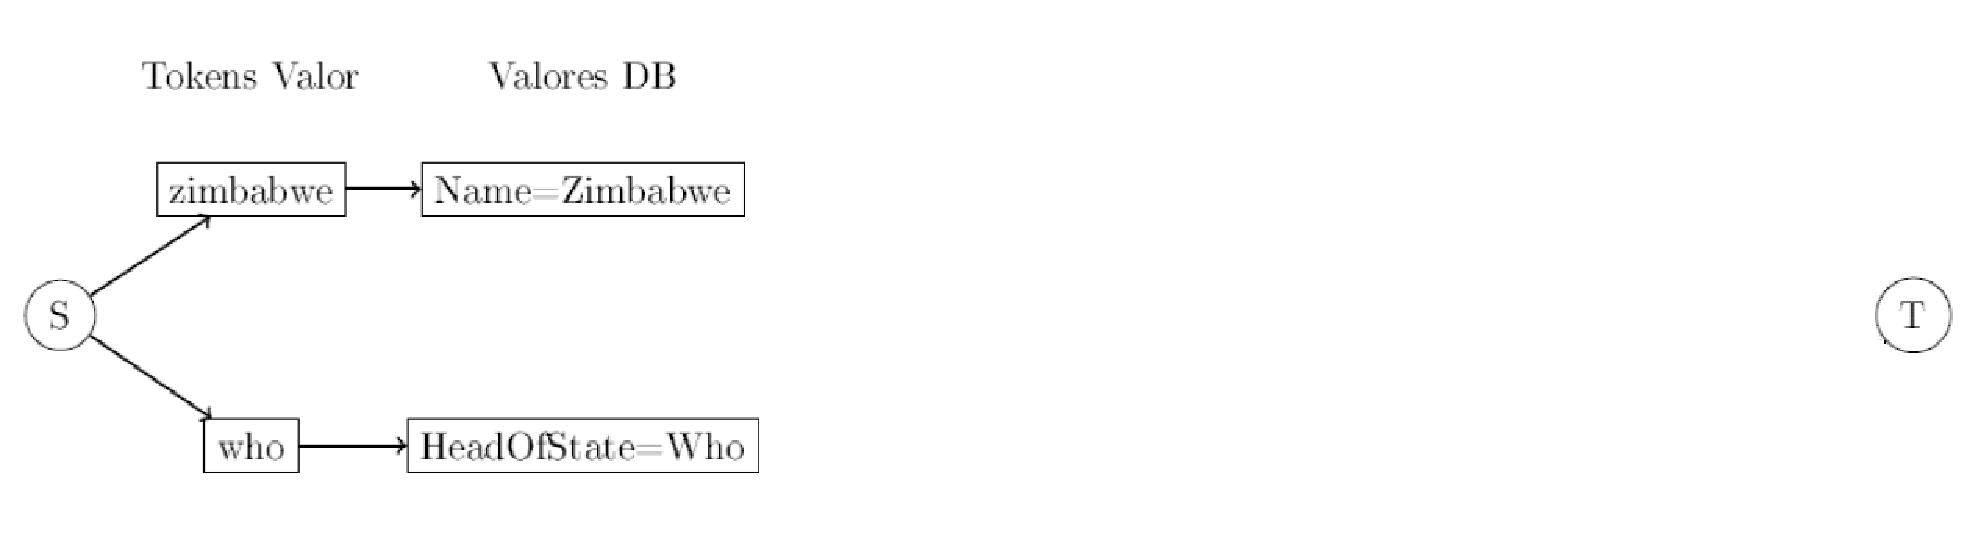
\includegraphics[scale=.33]{graficos/presentacion/ejemplo-grafo-matcher-1-4}
    \caption{3. Valores (DB) asociados a los tokens, con $f=1$}
\end{figure}
\end{frame}

\begin{frame}
\frametitle{Ejemplo 1: Matcher - Grafo de atributos y valores}
\begin{figure}
  \centering
    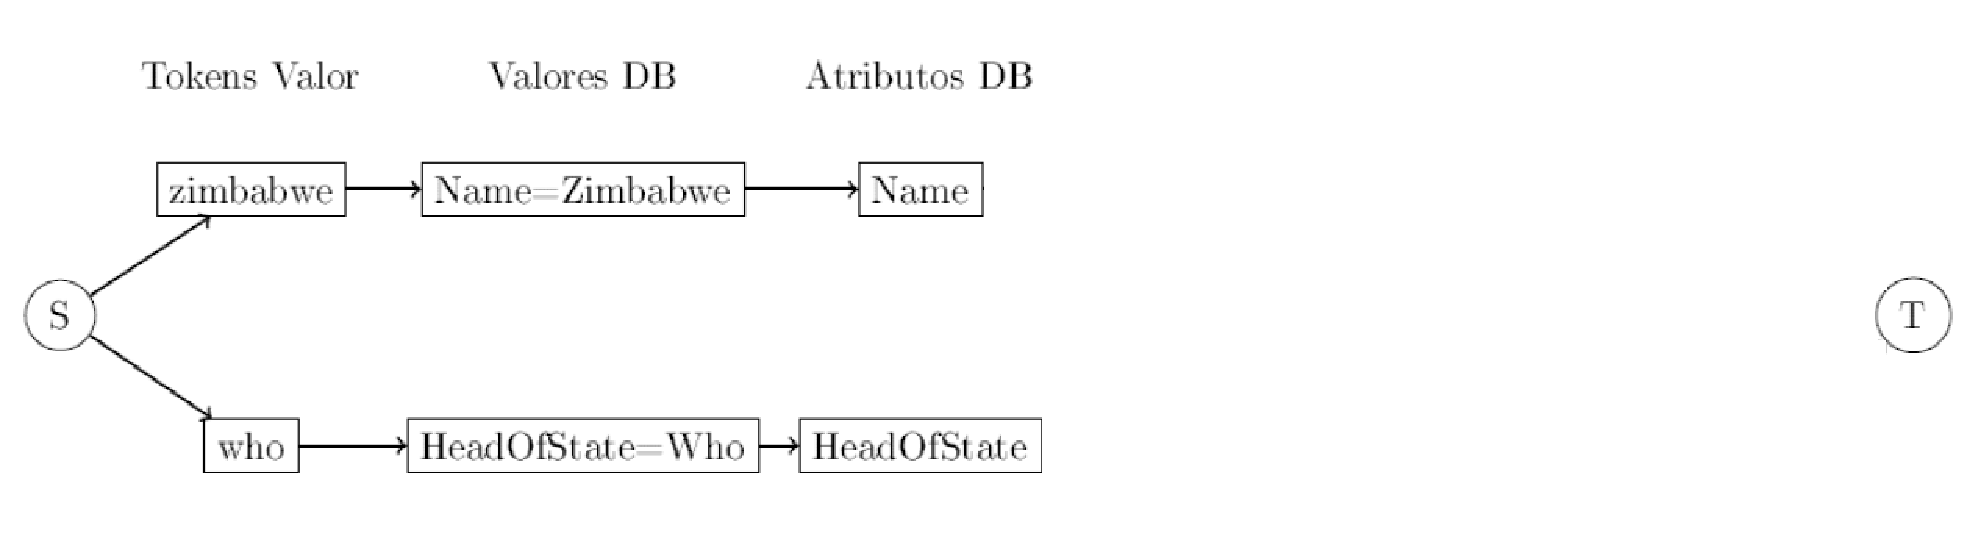
\includegraphics[scale=.33]{graficos/presentacion/ejemplo-grafo-matcher-1-5}
    \caption{4. Atributos (DB) asociados a los Valores, con $f=1$}
\end{figure}
\end{frame}

\begin{frame}
\frametitle{Ejemplo 1: Matcher - Grafo de atributos y valores}
\begin{figure}
  \centering
    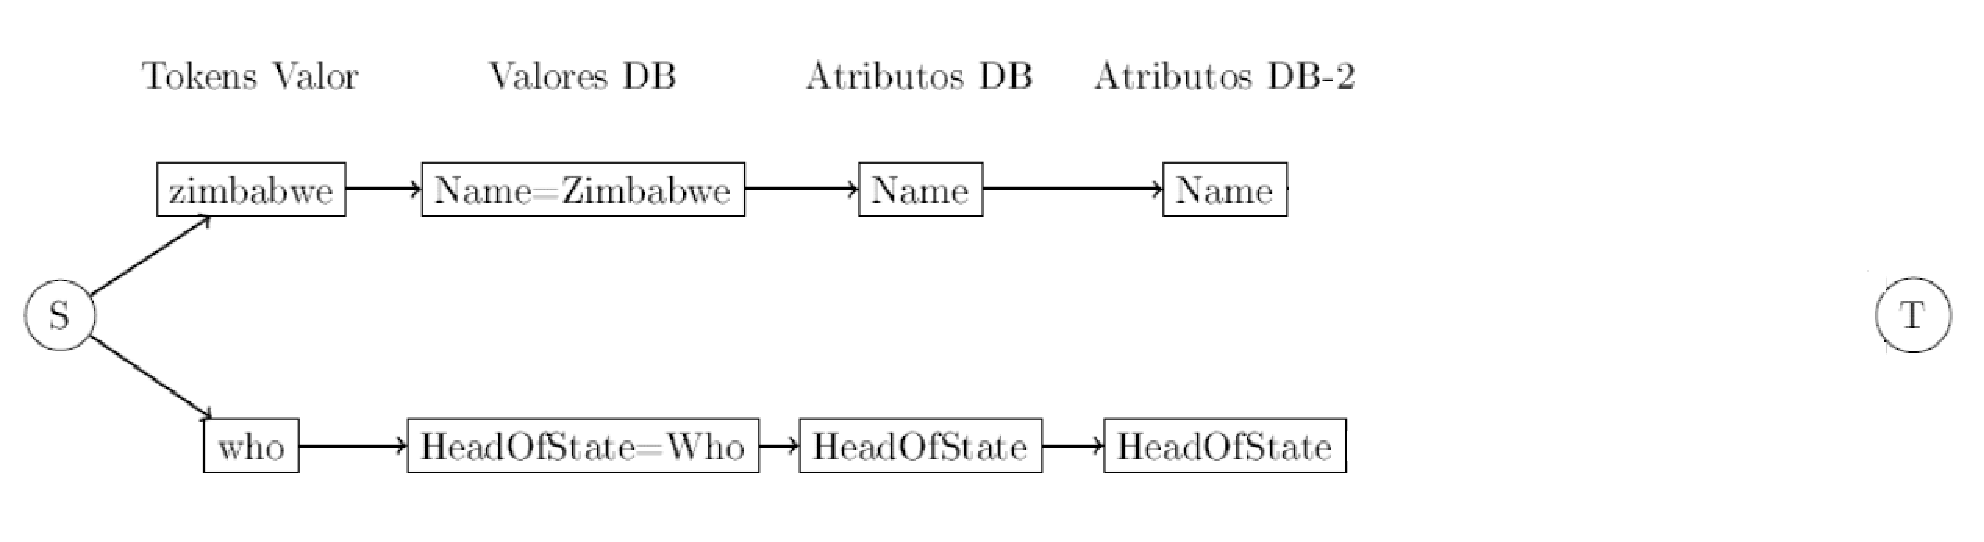
\includegraphics[scale=.33]{graficos/presentacion/ejemplo-grafo-matcher-1-5-2}
    \caption{5. Repite Atributos, para forzar $f=1$ por Atributo}
\end{figure}
\end{frame}

\begin{frame}
\frametitle{Ejemplo 1: Matcher - Grafo de atributos y valores}
\begin{figure}
  \centering
    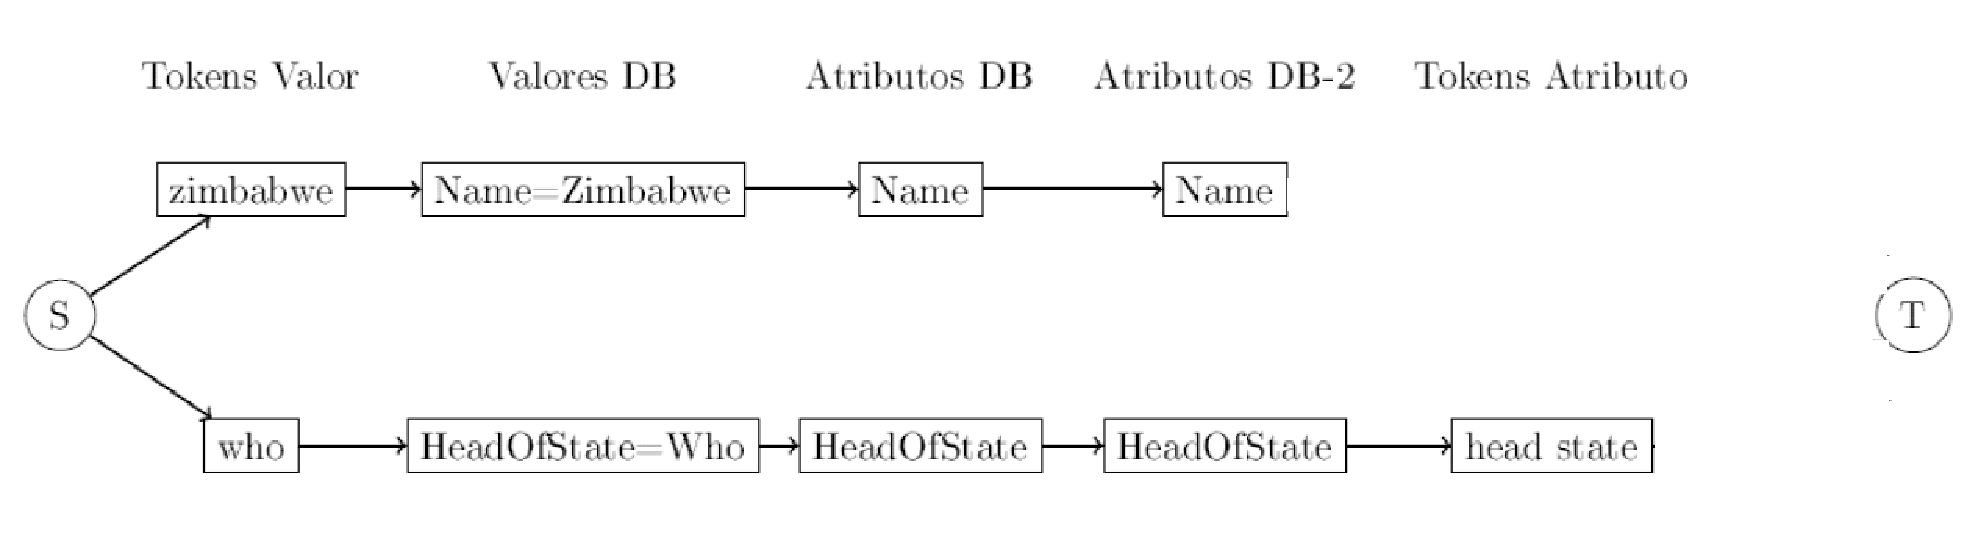
\includegraphics[scale=.33]{graficos/presentacion/ejemplo-grafo-matcher-1-5-3}
    \caption{6. Tokens de atributo, linkeados a Atributos con $f=1$}
\end{figure}
\end{frame}

\begin{frame}
\frametitle{Ejemplo 1: Matcher - Grafo de atributos y valores}
\begin{figure}
  \centering
    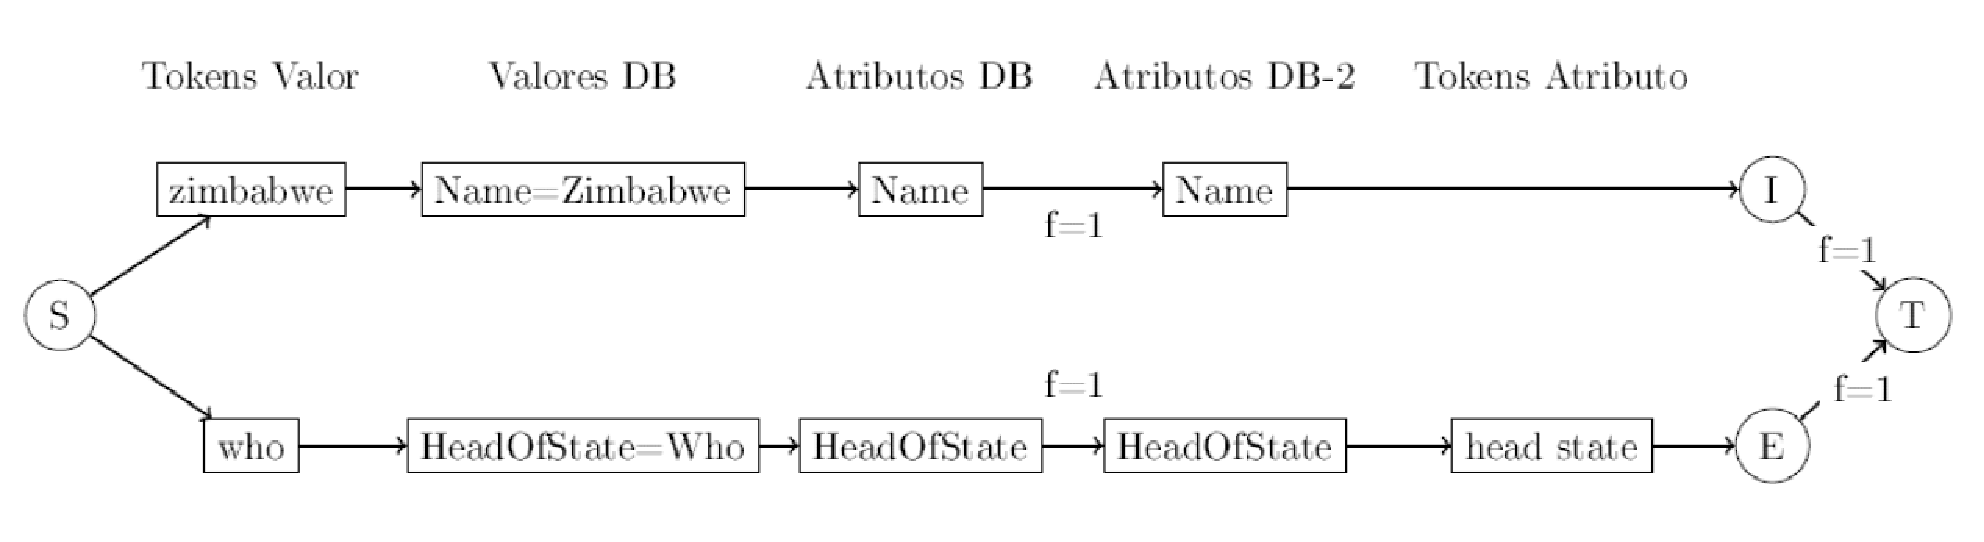
\includegraphics[scale=.33]{graficos/presentacion/ejemplo-grafo-matcher-1-6}
    \caption{6. Nodos I y E, con $f=tokens_{attr}$ y $f=tokens_{val} - tokens_{attr}$}
\end{figure}
\end{frame}


\begin{frame}[t]
\frametitle{Ejemplo 1: Matcher - notas}
\Large{``{\color{blue}Who} \st{is} \st{the} {\color{blue}head} \st{of} {\color{blue}state} \st{of} {\color{red}Zimbabwe}?''}
\normalsize{
\begin{itemize}
  \item {\color{blue}head state} es el atributo {\color{blue}Country.HeadOfState}
  \item {\color{blue}Who} es un valor (especial) de {\color{blue}Country.HeadOfState}
  \item {\color{red}Zimbabwe} es un valor de Country.Name ({\color{red}implícito})
  \item No desambigua nada (los tokens tiene un solo elemento asociado)
\end{itemize}
}
\bigskip
Los tokens de atributo y de valor explícitos apareados (`who' y `head state') deben estar sintácticamente asociados

\end{frame}
\begin{frame}[t]
\frametitle{Ejemplo 1: Matcher - Asociación sintáctica - Regla 1}
\Large{Regla 1: who $\rightarrow$ head}
\begin{center}
\begin{figure}
  \centering
    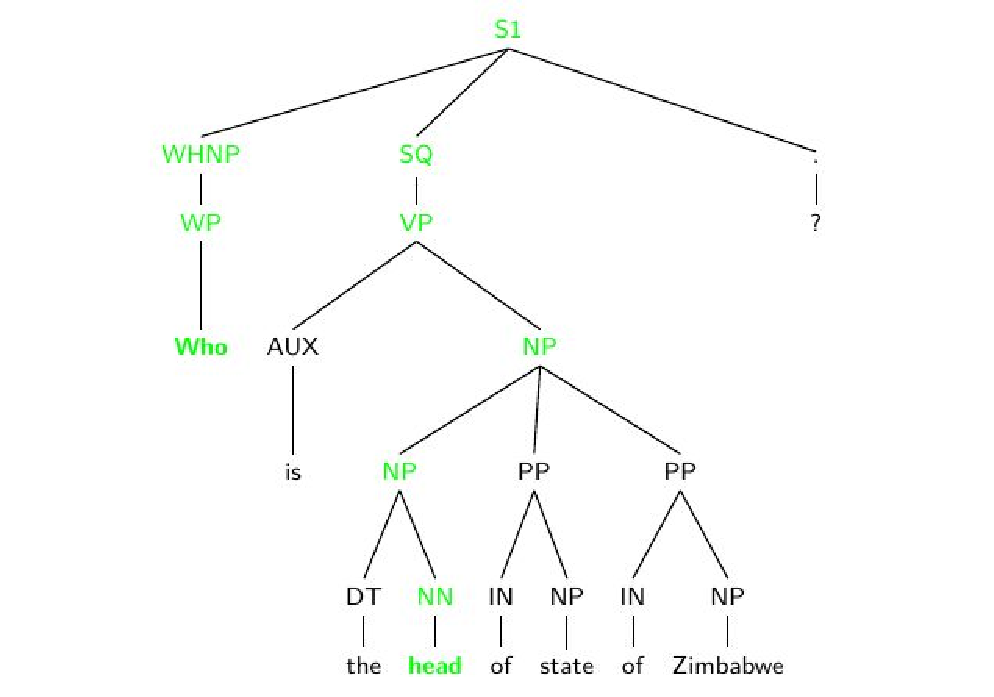
\includegraphics[scale=.5]{graficos/presentacion/ejemplo-charniak-2}
\end{figure}

\end{center}
\end{frame}

\begin{frame}[t]
\frametitle{Ejemplo 1: Matcher - Asociación sintáctica - Regla 6}
\Large{Regla 6: head $\rightarrow$ state}
\begin{center}

\begin{figure}
  \centering
    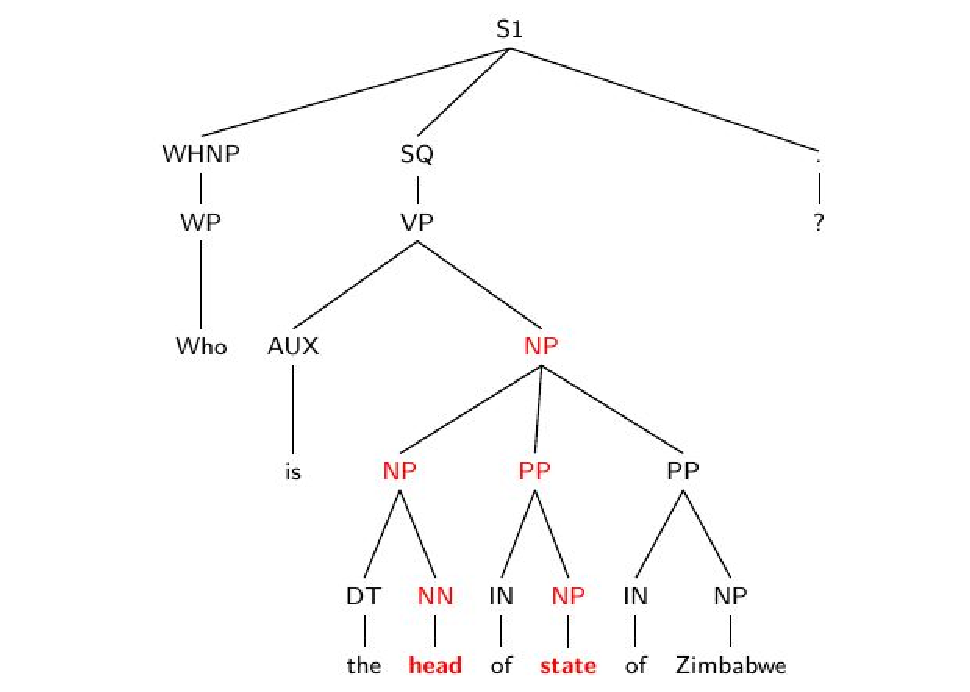
\includegraphics[scale=.5]{graficos/presentacion/ejemplo-charniak-1}
\end{figure}
\end{center}
\end{frame}

\begin{frame}[t]
\frametitle{Ejemplo 1: Generador de Queries}
\Large{{\color{blue}Who} \st{is} \st{the} {\color{blue}head} \st{of} {\color{blue}state} \st{of} {\color{red}Zimbabwe}? 
\bigskip
\newline
{\color{white}\textbf{{\color{white}SELECT}} HeadOfState \newline
{\color{white}\textbf{FROM}} Country \newline
{\color{white}\textbf{WHERE}} Country.Name$=$ {\color{white}`Zimbabwe'}
}}

\bigskip

{\color{white}\textbf{``Robert G. Mugabe''}}

\end{frame}

\begin{frame}[t]
\frametitle{Ejemplo 1: Generador de Queries}
\Large{{\color{blue}Who} \st{is} \st{the} {\color{blue}head} \st{of} {\color{blue}state} \st{of} {\color{red}Zimbabwe}? 
\bigskip
\newline
\textbf{{\color{blue}Who}} $\rightarrow$ Valor de Country.HeadOfState \newline
\textbf{{\color{blue}head state}} $\rightarrow$ Atributo Country.HeadOfState \newline
\textbf{{\color{red}Zimbabwe}} $\rightarrow$ Valor implícito de Country.Name \newline
}

\bigskip

{\color{white}\textbf{``Robert G. Mugabe''}}

\end{frame}

\begin{frame}[t]
\frametitle{Ejemplo 1: Generador de Queries}
\Large{{\color{blue}Who} \st{is} \st{the} {\color{blue}head} \st{of} {\color{blue}state} \st{of} {\color{red}Zimbabwe}? 
\bigskip
\newline
\textbf{{\color{purple}SELECT}} HeadOfState \newline
{\color{purple}\textbf{FROM}} Country \newline
{\color{purple}\textbf{WHERE}} Country.Name$=$ {\color{green}`Zimbabwe'}
}

\bigskip

\textbf{``Robert G. Mugabe''}

\end{frame}



\begin{frame}[<+->]
\frametitle{Ejemplo 2: What caribbean countries are also considered north american?}
  \begin{itemize}
    \item ``What caribbean countries are also considered north american?''
    \item Separar, puntuacion, lower case, lematizar, tirar stopwords: \newline \{what, caribbean, country, north, american\}
    \item Obtener tokens para cada lema y preservar solo los presentes en la pregunta:
      \begin{itemize}
        \item $getTokens(what)\ \rightarrow \{$'what'$\}$
        \item $getTokens(caribbean)\ \rightarrow \{$'caribbean'$\}$
        \item $getTokens(country)\ \rightarrow  \{$'country'$\}$
        \item $getTokens(north)\ \rightarrow \{$'north american'$\}$
        \item $getTokens(american)\ \rightarrow \{$'north american', 'american'$\}$
      \end{itemize}
  \end{itemize}
  
\end{frame}
\begin{frame}[<+->]
\frametitle{Ejemplo 2: Tokenizer}

  \begin{itemize}
  \item Generar tokenizaciones posibles:
    \begin{itemize}
      \item    \{ $\emptyset$, \{'north american'\}, \{'what', 'american', 'country'\}, \{'north american', 'what', 'american', 'country'\}, \{'american', 'caribbean'\}, ...\}
    \end{itemize}
  \item Quedarse con los no repetidos que cubren la pregunta (tokenizaciones completas): \{'north american', 'what', 'caribbean', 'country'\}
    \begin{itemize}
        \item Queda eliminado el token 'american'.
    \end{itemize}
  \end{itemize}

\end{frame}

\begin{frame}[<+->]
\frametitle{Lexicón: Tokens $\rightarrow$ Elementos DB}
Se obtienen todos los elementos que \textit{corresponden} a cada token:
   \small{
  \begin{itemize}

    \item caribbean $\rightarrow$ Caribbean (Valor de Country.Region \textbf{y} Valor de Country.Continent)
    \item north america $\rightarrow$ North America (Valor de Country.Continent)
    \item country $\rightarrow$ Country (Relación)
    \item what $\rightarrow$ What (Q-valor \textit{compatible} con un montón de Atributos)
    
  \end{itemize}
  }
\end{frame}

\begin{frame}
\frametitle{Matcher: Grafo atributo-valor}
\begin{figure}
  \centering
    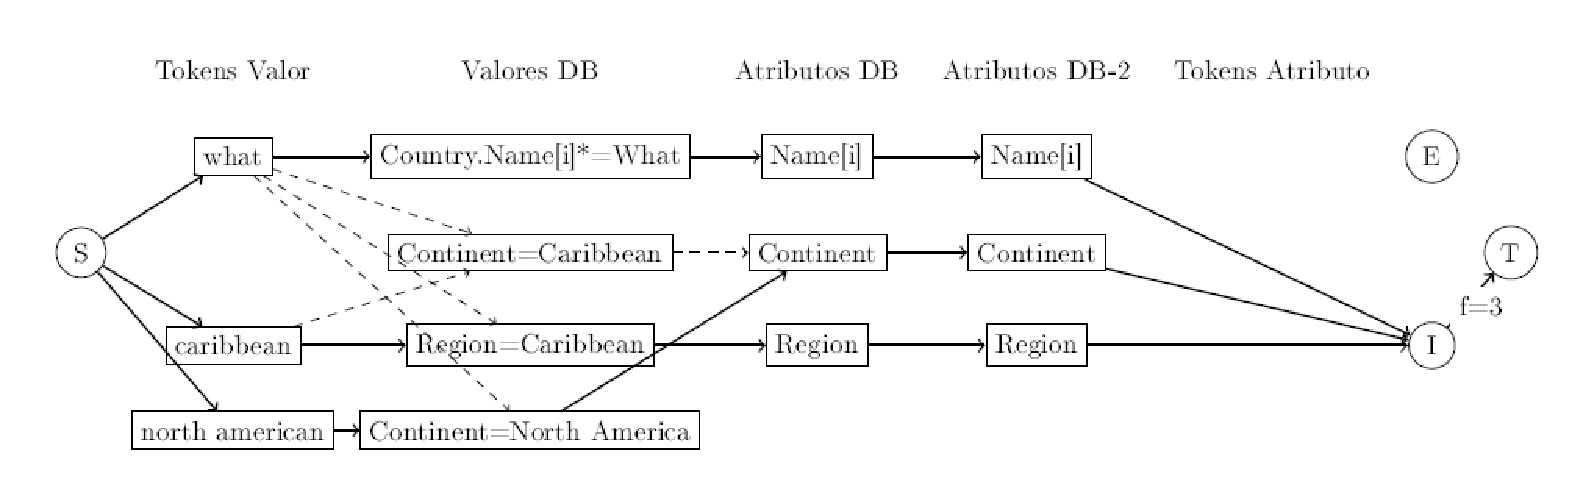
\includegraphics[scale=.43]{graficos/presentacion/ejemplo-grafo-2}
    \caption{Grafo con desambiguación}
\end{figure}

Notar:
  \begin{itemize}
    \item Caribbean es ambigüo.
    \item Como north american solo puede ser Continent, caribbean va a ser Region (para maximizar el flujo)
  \end{itemize}
\end{frame}

\begin{frame}[<+->]
\frametitle{Ejemplo 2: Query}
Query final:\newline
\Large{\textbf{{\color{purple}SELECT DISTINCT} Country.Name \newline{\color{purple}FROM} Country \newline{\color{purple}WHERE} Country.Continent $=$ {\color{green}'North America'} \newline{\color{purple}AND} Country.Region $=$ {\color{green}'Caribbean'}}}

\end{frame}



\begin{frame}
\frametitle{Corridas}
Corridas sobre 200 preguntas escritas a mano para testing
\begin{center}
\begin{table}[h]
\centering
\begin{tabular}{| r |  p{12cm} | }

Total & Categoría \\ 
91 & Respuesta exacta \\ 
27 & Ambiguas inherentemente + pedido de reformulación \\ 
11 & Sin respuesta (razonable, fuera de scope) \\
32 & Fallas simples en stopwords o en lexicón \\
10 & Ambiguas por problemas de sinonimia en el modelo \\
4 & Ambiguas. Problemas del lexicón. \\
6 & El analizador sintáctico no encontró asociación. \\
19 & Problemáticas. Análisis más detallado en texto. \\
200 & Total \\
\end{tabular}
\caption{Resultados de la primera corrida sobre las preguntas de test}
\label{table:popescu-results-1}
\end{table}
\end{center}
\end{frame}

\begin{frame}
\frametitle{Corridas}
Después de correcciones pavas:
\begin{center}
\begin{table}[h]
\centering
\begin{tabular}{| r |  p{12cm} |}
Total & Categoría \\ 
126 & Respuesta exacta \\ 
38 & Ambiguas \\ 
36 & Sin respuesta\\ 
200 & Total \\ 

\end{tabular}
\caption{Resultados sobre las preguntas de test (con correcciones)}
\label{table:popescu-results-3}
\end{table}
\end{center}
\end{frame}


\subsubsection*{Conclusiones y limitaciones}

\begin{frame}
\frametitle{Conclusiones y limitaciones: dominio cerrado}
Mejoras / trabajo futuro
\begin{itemize}
\item Generación del Lexicón
\item Desambiguador de sentidos para los sinónimos de los tokens
\item Generación de Stopwords
\item Soportar diferentes paths para aparear (\textit{joinear}) tablas.
%\item Soportar tokens multi tipados en el Matcher.
%\item Soportar desambiguación de relaciones en el Matcher.
\item Interfaz con el usuario: SQL $\rightarrow$ respuesta
\item CharniakParseTree: evaluar con un lingüista profesional las reglas

\end{itemize}
\end{frame}


\begin{frame}
\frametitle{Conclusiones y limitaciones: dominio cerrado}

\begin{itemize}
  \item Hipótesis fecunda del modelo: subset de preguntas. Tratabilidad semántica.
  \begin{itemize}
    \item \textit{Zonas} computables del lenguaje
  \end{itemize}
  \item Modelo potente pero subespecificado (sinónimos, stopwords, attachment)
  \item La implementación requiere desarrollo humano dedicado y tuneo
  \item Killer combo con text-to-speech
  \end{itemize}

\end{frame}




